\documentclass{article}
\usepackage[utf8]{inputenc}
\usepackage{amsmath}
\usepackage[linesnumbered,ruled]{algorithm2e}
\usepackage{mathtools}
\usepackage{commath}
\usepackage{bm}
\usepackage{hyperref}
\usepackage{tikz}
\usepackage{placeins}
\usepackage{listings}
\usetikzlibrary{shapes.geometric, arrows}

\title{Report of Puyuma self-driving system\\  Lane following algorithm}
\author{\textbf{Sheng-Wen Cheng , Po-Sheng Chen}}
\date{August 2019}

\begin{document}

\maketitle

\tikzstyle{blocks} = [rectangle, rounded corners, minimum width=2cm, minimum height=1cm,text centered, draw=black, fill=orange!30]
\tikzstyle{arrow} = [thick,->,>=stealth]

\section{Introduction}
Puyuma is a computer vision based self-driving system inspired by MIT duckietown project. By using Xenomai Linux real-time extension, we had created a miniature self-driving system which is suitable for doing real-time robotics research.
\\
\\
This report introduces the design of Puyuma self-driving system, including computer vision algorithm, data filtering and controller design.
\\
\\
\\
\\

\begin{figure}[ht]
  \label{fig:xenobot}
  \centering
  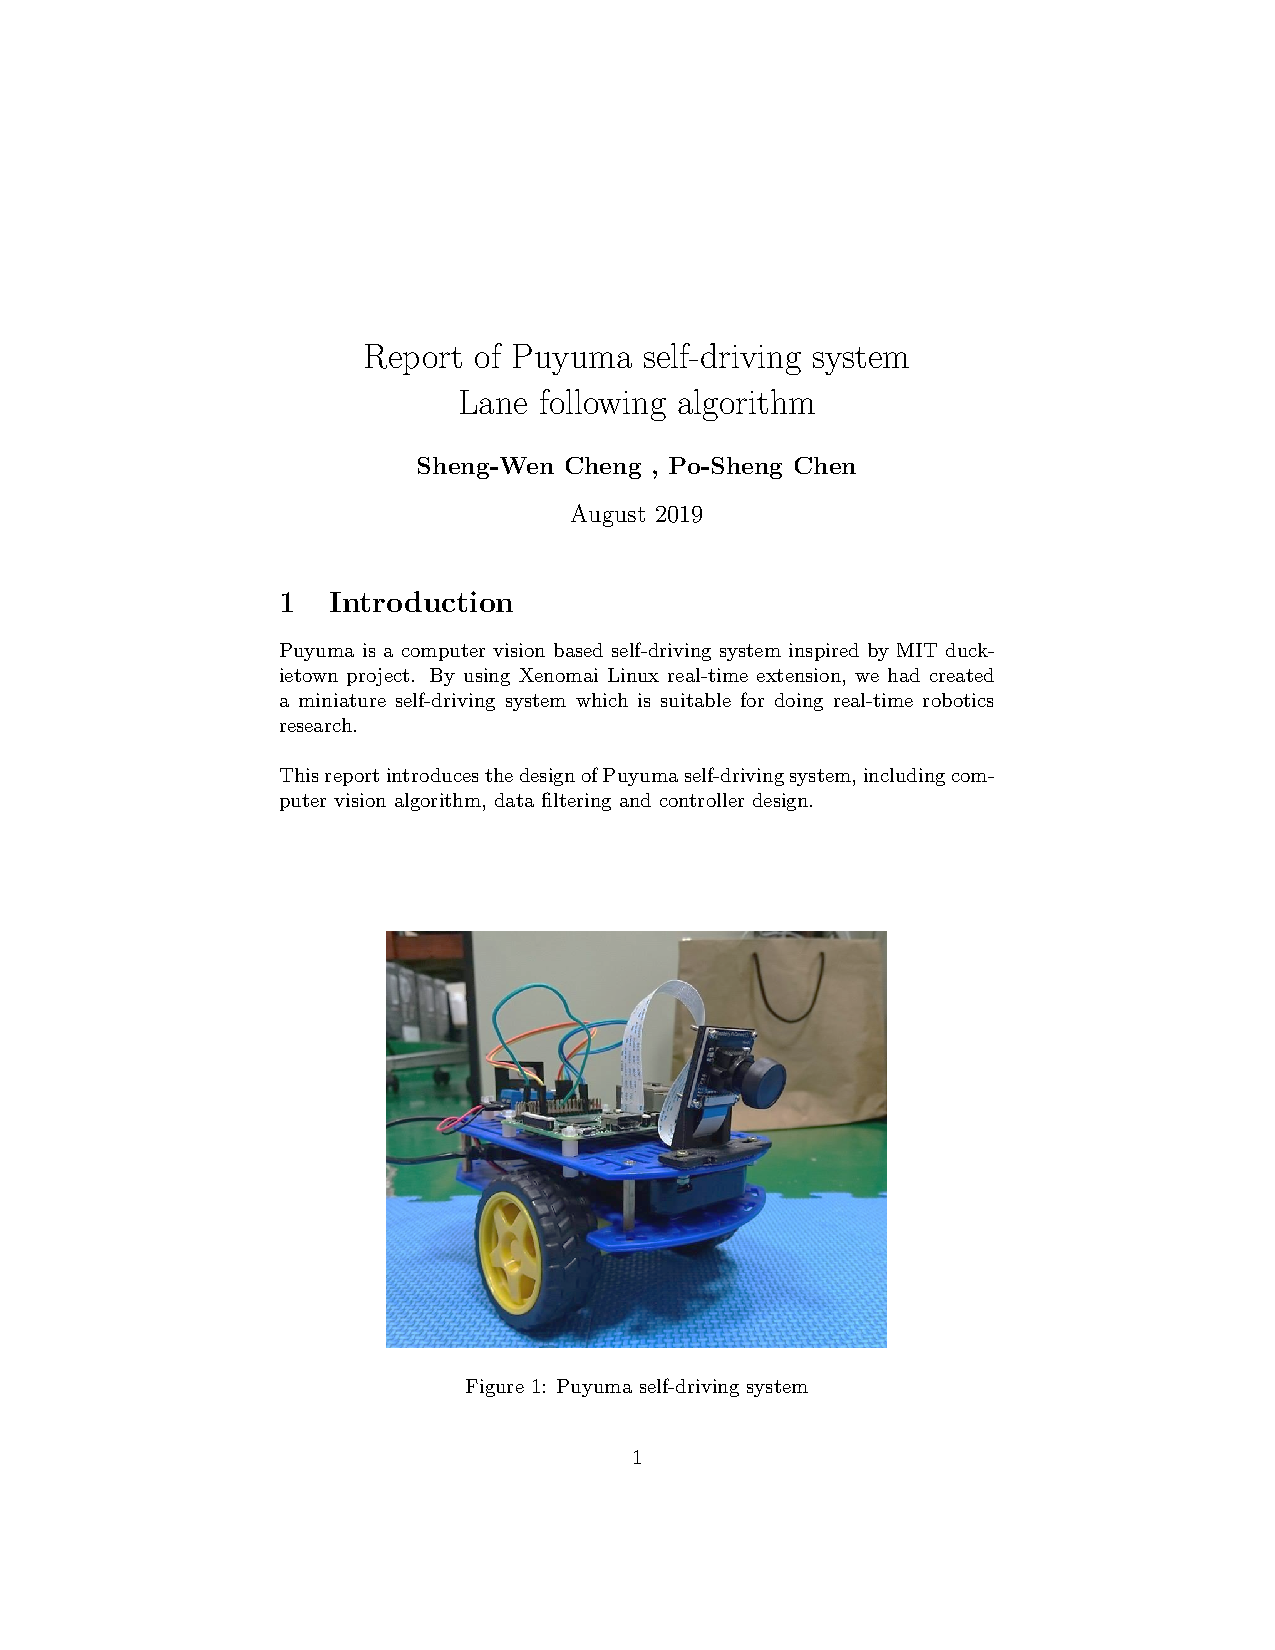
\includegraphics[scale=0.3]{graphs/xenobot.PNG}
  \caption{Puyuma self-driving system}
\end{figure}

\clearpage

\section{Camera calibrations}

Camera calubration is a early stage job before running computer vision algorithm. There are two set of parameters need to be found, intrinsic parameters and extrinsic parameters. They describe the relation between 2D image plane and 3D world. 

\subsection{Intrinsic calibration}

Intrinsic matrix describes the 3D world to 2D image plane projection. The ideal linear camera model is consist of focal length, pixel size and principal point. Non-linear effects like lens distortion also exists but can not be modeled by linear equations, therefor it is usually solved by numerical methods.

\begin{figure}[ht]
  \label{fig:distortion}
  \centering
  \includegraphics[scale=0.3]{graphs/distortion.png}
  \caption{Camera undistortion and rectification}
\end{figure}
\FloatBarrier

\begin{figure}[ht]
  \label{fig:intrinsic_calibration}
  \centering
  \includegraphics[scale=0.5]{graphs/intrinsic_calibration.png}
  \caption{Intrinsic calibration}
\end{figure}
\FloatBarrier

\subsection{Extrinsic calibration}

Extrinsic matrix describes the translation and rotation of camera with respect to the world frame. ( i.e., angle and position of camera in 3D world.)

\begin{figure}[ht]
  \label{fig:extrinsic_calibration}
  \centering
  \includegraphics[scale=0.7]{graphs/extrinsic_calibration.png}
  \caption{Extrinsic calibration}
\end{figure}
\FloatBarrier

\clearpage

\section{Lane pose estimation}

\subsection{System conventions}

The coordination system of Puyuma self-driving system is defined as follow: x points to right, y points foward and z point upward.

\begin{figure}[ht]
  \label{fig:lane_coordination}
  \centering
  \includegraphics[scale=0.6]{graphs/coordinate_system.PNG}
  \caption{Lane coordination}
\end{figure}
\FloatBarrier

\noindent We also assume the car always drives between yellow and white line. The yellow line is called inner segment and located to the left.  The white line is called outer segment and located to the right.

\begin{figure}[ht]
  \label{fig:lane_2d_view}
  \centering
  \includegraphics[scale=0.6]{graphs/lane_parameter_2d_view.PNG}
  \caption{2D view of lane}
\end{figure}
\FloatBarrier

\noindent Now we can define the pose of the car: $\bm{d}$ is the lateral displacement and $\bm{\phi}$ is the orientation angle.


\begin{figure}[ht]
  \label{fig:lane_pose}
  \centering
  \includegraphics[scale=0.7]{graphs/lane_pose.PNG}
  \caption{Lane pose}
\end{figure}
\FloatBarrier

\subsection{Segements detection}

Before doing pose estimation, the lane segments have to be detected from image. Canny edge detection, HSV color thresholding and Hough transform are used.

\begin{figure} [ht]
\begin{center}
\begin{tikzpicture}[node distance=2cm]
\node (raw) [blocks, yshift=0cm] {Raw image} ;
\node (rectify) [blocks, yshift=-1.5cm] {Distortion and rectification};
\node (canny) [blocks, xshift=-2cm, yshift=-3cm] {Canny edge detection};
\node (diliation_canny) [blocks, xshift=-2cm, yshift=-4.5cm] {Diliation};
\node (threshold) [blocks, xshift=2cm, yshift=-3cm] {HSV color thresholding};
\node (diliation_threshold) [blocks, xshift=2cm, yshift=-4.5cm] {Diliation};
\node (and) [blocks, yshift=-6cm] {Bitwise AND operation};
\node (hough) [blocks, yshift=-7.5cm] {Hough transform};
\node (segments) [blocks, yshift=-9cm] {Segments};

\draw [arrow] (raw) -- (rectify);
\draw [arrow] (rectify) -- (canny);
\draw [arrow] (canny) -- (diliation_canny);
\draw [arrow] (rectify) -- (threshold);
\draw [arrow] (threshold) -- (diliation_threshold);
\draw [arrow] (diliation_canny) -- (and);
\draw [arrow] (diliation_threshold) -- (and);
\draw [arrow] (and) -- (hough);
\draw [arrow] (hough) -- (segments);
\end{tikzpicture}
\end{center}
\caption{Lane detector workflow}
\end{figure}
\FloatBarrier

\noindent The image is first transfromed from RGB color space into the HSV color space. Color thresholding method is then applied on HSV color space to find the interest color region like yellow or white.

\begin{figure}[ht]
  \label{fig:threshold}
  \centering
  \includegraphics[scale=0.5]{graphs/threshold.jpeg}
  \caption{Binary image of color thresholding result}
\end{figure}
\FloatBarrier

\noindent After the color thresholding step, Canny edge detection is applied as a preprocessing step of Hoght transform. By using Hough transform, the line position (point-to-point) vector can be obtained for further computation.

\begin{figure}[ht]
  \label{fig:canny}
  \centering
  \includegraphics[scale=0.5]{graphs/canny.jpeg}
  \caption{Result of Canny edge detection}
\end{figure}
\FloatBarrier

\noindent A bitwise AND operation of color thresholding image and Canny edge image is also used to to distinguish segements from different colors. The following figure shows the visualization result of lane segments and car pose: $d$ and $\phi$.

\begin{figure}[ht]
  \label{fig:hough}
  \centering
  \includegraphics[scale=0.5]{graphs/lane_mark.jpeg}
  \caption{A visualization image of lane pose estimator result}
\end{figure}
\FloatBarrier


\subsection{Frame transformation}

The camera is mounted in a certain distance from origin to the car. A camera-to-car frame coordinate transformation is needed for obtaining the right result.

\[
\begin{pmatrix} x_{car} \\ y_{car} \end{pmatrix} = 
\begin{pmatrix} x_{camera} - r \cdot \sin\phi \\ y_{camera} - r \cdot \cos\phi \end{pmatrix}
\]

\begin{figure}[ht]
  \label{fig:frame_transformation}
  \centering
  \includegraphics[scale=0.7]{graphs/frame_transformation.PNG}
  \caption{Frame transformation}
\end{figure}
\FloatBarrier

\subsection{Segment side recognition}

Although the lane detector can help for finding segments, a segment side recognizing algorithm is also needed. We can determine the left or right side by testing several pixels in positive and negative direction on the lane segment normal vector direction. (using color thresholding image)
\\
\\

\begin{figure}[ht]
  \label{fig:lane_segment}
  \centering
  \includegraphics[scale=0.4]{graphs/segment.PNG}
  \caption{Segment side recognition}
\end{figure}
\FloatBarrier

\begin{figure} [ht]
\begin{algorithm}[H]
	\KwData{segment, accumulator threshold, color binarization image}
	\KwResult{side (left or right)}
	$\vec{P_1} = (x_1, y_1)$

	$\vec{P_2} = (x_2, y_2)$

	$\vec{P} = (\vec{P_1} + \vec{P_2}) / 2$

	$\vec{t} = \frac{\vec{P_2} - \vec{P_1}}
					{\norm{\vec{P_2} - \vec{P_1}}}$

	$\vec{n} = (-y_t, x_t)$

	$left \gets 0 \ , \ right \gets 0$

	\For {$i < pixel \ count$} {
		$x \gets \lceil x_p + x_n \cdot i \rceil$

		$y \gets \lceil y_p + y_n \cdot i \rceil$
	
		\uIf{$I(x,y) = I_{max}$}
			{
				$left \mathrel{+}= 1$ 
			}
			
		$x \gets \lfloor x_p - x_n \cdot i \rfloor$

		$y \gets \lfloor y_p - y_n \cdot i \rfloor$
		
		\uIf{$I(x,y) = I_{max}$}
			{
				$right \mathrel{+}= 1$ 
			}
	}
	
	\uIf {$left > threshold \ \& \  right < threshold$}
		{
			\Return is\_left
		}
	\uElseIf {$right > threshold \ \& \ left < threshold$}
		{
			\Return is\_right
		}
	\uElse
		{
			\Return unknown side
		} 
	\caption{Segment side recognizing algorithm}
\end{algorithm}
\end{figure}
\FloatBarrier

\subsection{Ground projection}

During the calibration stage, we already found the homography matrix which can help us map the image from camera's perspection to bird view perspection. This is usally called inverse perspective mapping. Inverse perspective mapping is applied before running the lane detector algorithm

\begin{figure}[ht]
  \label{fig:ground projection}
  \centering
  \includegraphics[scale=0.7]{graphs/ground_project.png}
  \caption{Ground projection}
\end{figure}
\FloatBarrier

\subsection{Pose estimation for single segment}

Each segments detected by lane detector detects can be treated as a single pose data due to the lane geometry. These datas are put into a histogram filter for data filitering later. The process acts like a voting mechanism so is called a vote generating function.

\begin{figure}[ht]
  \label{fig:lane_geometry}
  \centering
  \includegraphics[scale=1]{graphs/lane_geometry.PNG}
  \caption{Lane geometry}
\end{figure}
\FloatBarrier

\begin{figure} [ht]
\begin{algorithm}[H]
	\KwData{segment}
	\KwResult{pose $d_{i}$ and $\phi_{i}$}
	$\vec{P_1} = (x_1, y_1)$

	$\vec{P_2} = (x_2, y_2)$

	$\vec{t} = \frac{\vec{P_2} - \vec{P_1}}
					{\norm{\vec{P_2} - \vec{P_1}}}$

	$\vec{n} = (-y_t, x_t)$

	$\phi_{i} = \arctan(\frac{y_t}{x_t}) - \pi / 2$

	\uIf {segment color = white}
		{
			\eIf{edge side = right}
			{
				$\vec{k} = (\frac{w}{2} + l_w) \cdot \vec{n}$
			}
			{
				$\vec{k} = (\frac{w}{2}) \cdot \vec{n}$
			}
		}
	\uElseIf {segment color = yellow}
		{
			\eIf{edge side = left}
			{
				$\vec{k} = (-\frac{w}{2} - l_y) \cdot \vec{n}$
			}
			{
				$\vec{k} = (-\frac{w}{2}) \cdot \vec{n}$
			}
		}
	$\vec{j} = (r \cdot \sin\phi, r \cdot \cos\phi)$

	$\vec{P_1^\prime} = \vec{P_1} + \vec{k} - \vec{j}$

	$\vec{P_2^\prime} = \vec{P_2} + \vec{k} - \vec{j}$

	$d_1 = \vec{P_1} \cdot \vec{n}$

	$d_2 = \vec{P_2} \cdot \vec{n}$

	$d_{i} = (d_1 + d_2) / 2$
	\caption{Vote generating function}
\end{algorithm}
\end{figure}
\FloatBarrier

\subsection{Histogram filter}

Segment poses generated in previous process are then collected into the histogram filter. The histogram filter is designed to find the \textbf{mode} of datas and eliminate extremes.
\\
\\
\noindent After the process, The \textbf{mean} of pose datas is calculated and becomes the estimation result.

\begin{figure}[ht]
  \label{fig:histogram_filter}
  \centering
  \includegraphics[scale=0.9]{graphs/histogram_filter.PNG}
  \caption{Histogram filter}
\end{figure}
\FloatBarrier

\begin{figure} [ht]
\begin{algorithm}[H]
	\KwData{segment}
	\KwResult{filtered pose $d$ and $\phi$}
	\For {$\bm{all}$ segments} {
			$(\phi_i, d_i) \gets generate\_vote(segment)$
			
			$I \gets round(\frac{\phi_i - \phi_{min}}{\Delta\phi})$

			$J \gets round(\frac{d_i - d_{min}}{\Delta d})$
			
			$histogram(I, J) \mathrel{+}= 1$
	}
	
	$(I_{highest}, J_{highest}) \gets find \_ highest \_ vote()$	
	
	$\phi_{histogram} \gets I_{highest} \cdot \Delta \phi + \phi_{min}$
	
	$d_{histogram} \gets J_{highest} \cdot \Delta d + d_{min}$

	$\phi_{mean} \gets 0 \ , \  d_{mean} \gets 0$
	
	$N_{\phi} \gets 0 \ , \ N_{d} \gets 0$
	
	\For {$\bm{all} \ (\phi_{i}, d_{i})$}
	{
		\uIf {$\phi_{i} \in [\phi_{histogram} - \frac{\Delta \phi}{2}, 
			  \phi_{histogram} + \frac{\Delta \phi}{2}]$}
		{
			$\phi_{mean} \mathrel{+}= \phi_{i}$
			
			$N_{\phi} \mathrel{+}= 1$
		}
		
		\uIf {$d_{i} \in [d_{histogram} - \frac{\Delta d}{2}, 
			  d_{histogram} + \frac{\Delta d}{2}]$}
		{
			$d_{mean} \mathrel{+}= d_{i}$
			
			$N_{d} \mathrel{+}= 1$
		}
	}
	
	$\phi_{mean} \gets \frac{\phi_{mean}}{N_{\phi}}$
	
	$d_{mean} \gets \frac{d_{mean}}{N_{d}}$	
	\caption{Histogram filter}
\end{algorithm}
\end{figure}
\FloatBarrier

\clearpage

\section{Control system design}

\subsection{Differential wheels}

Puyuma is designed as a differential wheeled robot. There are two independent motors on the car. The car can turn by changing the speed rate between two motors. Hence it does not require any additional steering mechanism.

\begin{figure}[ht]
  \label{fig:ground projection}
  \centering
  \includegraphics[scale=0.7]{graphs/differential_wheels.PNG}
  \caption{Differential wheeled robot}
\end{figure}
\FloatBarrier

\subsection{PID Controller}

We use the well known algorithm \textbf{"PID controller"} to fix the orientation and lateral displacement error.
\\
\\
The equation of PID controller in continuous time is given as:

\[e(t) = setpoint(t) - x(t)\]

\[u(t) = K_p e(t) + K_i \int_{0}^{t} e(\tau) d\tau + K_d  \frac{de(t)}{dt}\]

\noindent and for discreted time:

\[e[t] = setpoint[t] - x[t]\]

\[u[t] = K_p e[t] + K_i \sum_0^t e[t] \Delta t + K_d \frac{e[t] - e[t-1]}{\Delta t}\]

\subsection{Pose control}

The pose controller of Puyuma is designed as a cascaded PID controller.
\\
\\
We designed phi controller as a lower level contoller for orientation stablizing. d controller can fix the lateral displacement error by changing phi controller's setpoint to turn left or right.

\begin{figure}[ht]
  \label{fig:control_diagram}
  \centering
  \includegraphics[scale=0.6]{graphs/control_diagram.PNG}
  \caption{Control diagram}
\end{figure}
\FloatBarrier

\noindent The wheel control signal (PWM) are simply the throttle value plus/minus the correction value:

\begin{lstlisting}
pwm_left = THROTTLE__BASE - pwm_correction
pwm_right = THROTTLE__BASE + pwm_correction
\end{lstlisting}

\clearpage

\section{References}

[1] Lane Filter by Liam Paull, MIT CSAIL

\end{document}